\documentclass[a4paper,10pt]{article}
\usepackage[utf8]{inputenc}
\usepackage{graphicx}
\usepackage{titling}
% Title Page
\title{Rapport projet 2}
\author{Joël Felderhoff, Louis Bethune}


\begin{document}

\pretitle{%
  \begin{center}
  \LARGE
  
\includegraphics{notre_projet.jpg}\\[\bigskipamount]
}

\posttitle{\end{center}}
\maketitle

\section{Notes concernant le typage}
Un choix de conception a été fait concernant le typage des variables. Le choix est le suivant : la sémantique l'emporte toujours.
Typiquement, les littéraux sont représenté par un type précis : \textbf{Var(x)} à la place de juste utiliser des entiers.

Ce choix induit une certaine lourdeur à la programmation mais est justifié par le fait que un typage marqué diminue de manière importante les erreurs de programmation : 
il n'y aurait aucun intéret à additionner deux littéraux par exemple, c'est donc rendu impossible.

\section{Le type ROBDD}
Réalisé conjointement par Louis Bethune et Joël Felderhoff

Ce type est un type d'arbre tout ce qui a de plus classique. Le partage est fait grâce à un foncteur prenant en paramètre un type de dictionnaire.
J'ai (Joël) réalisé le dictionnaire utilisant des tables de hachages sur les littéraux, contenant la liste des noeuds dépendant de chaque littéraux.

Nous avons donc une complexité en O(nombre de noeuds pour un littéral donné).

Une amélioration pourrait être réalisée en hachant directement les noeuds (par exemple avec une fonction standard de OCaml).

\section{Benchmark}
Réalisé par Joël Felderhoff.

J'ai réalisé un petit script python générant une formule aléatoire et faisant, à l'aide d'une boucle, des moyennes des temps d'exécutions.

Le graphique suivant a été réalisé avec matplotlib, et représente le temps d'exécution moyen (sur 50 tests) en seconde de l'exécution du programme (création de la robdd et sifting) en fonction du nombre de
connecteurs logiques dans le programme (on a $x$ littéraux pour $4x$ connecteurs logiques).

\begin{center}
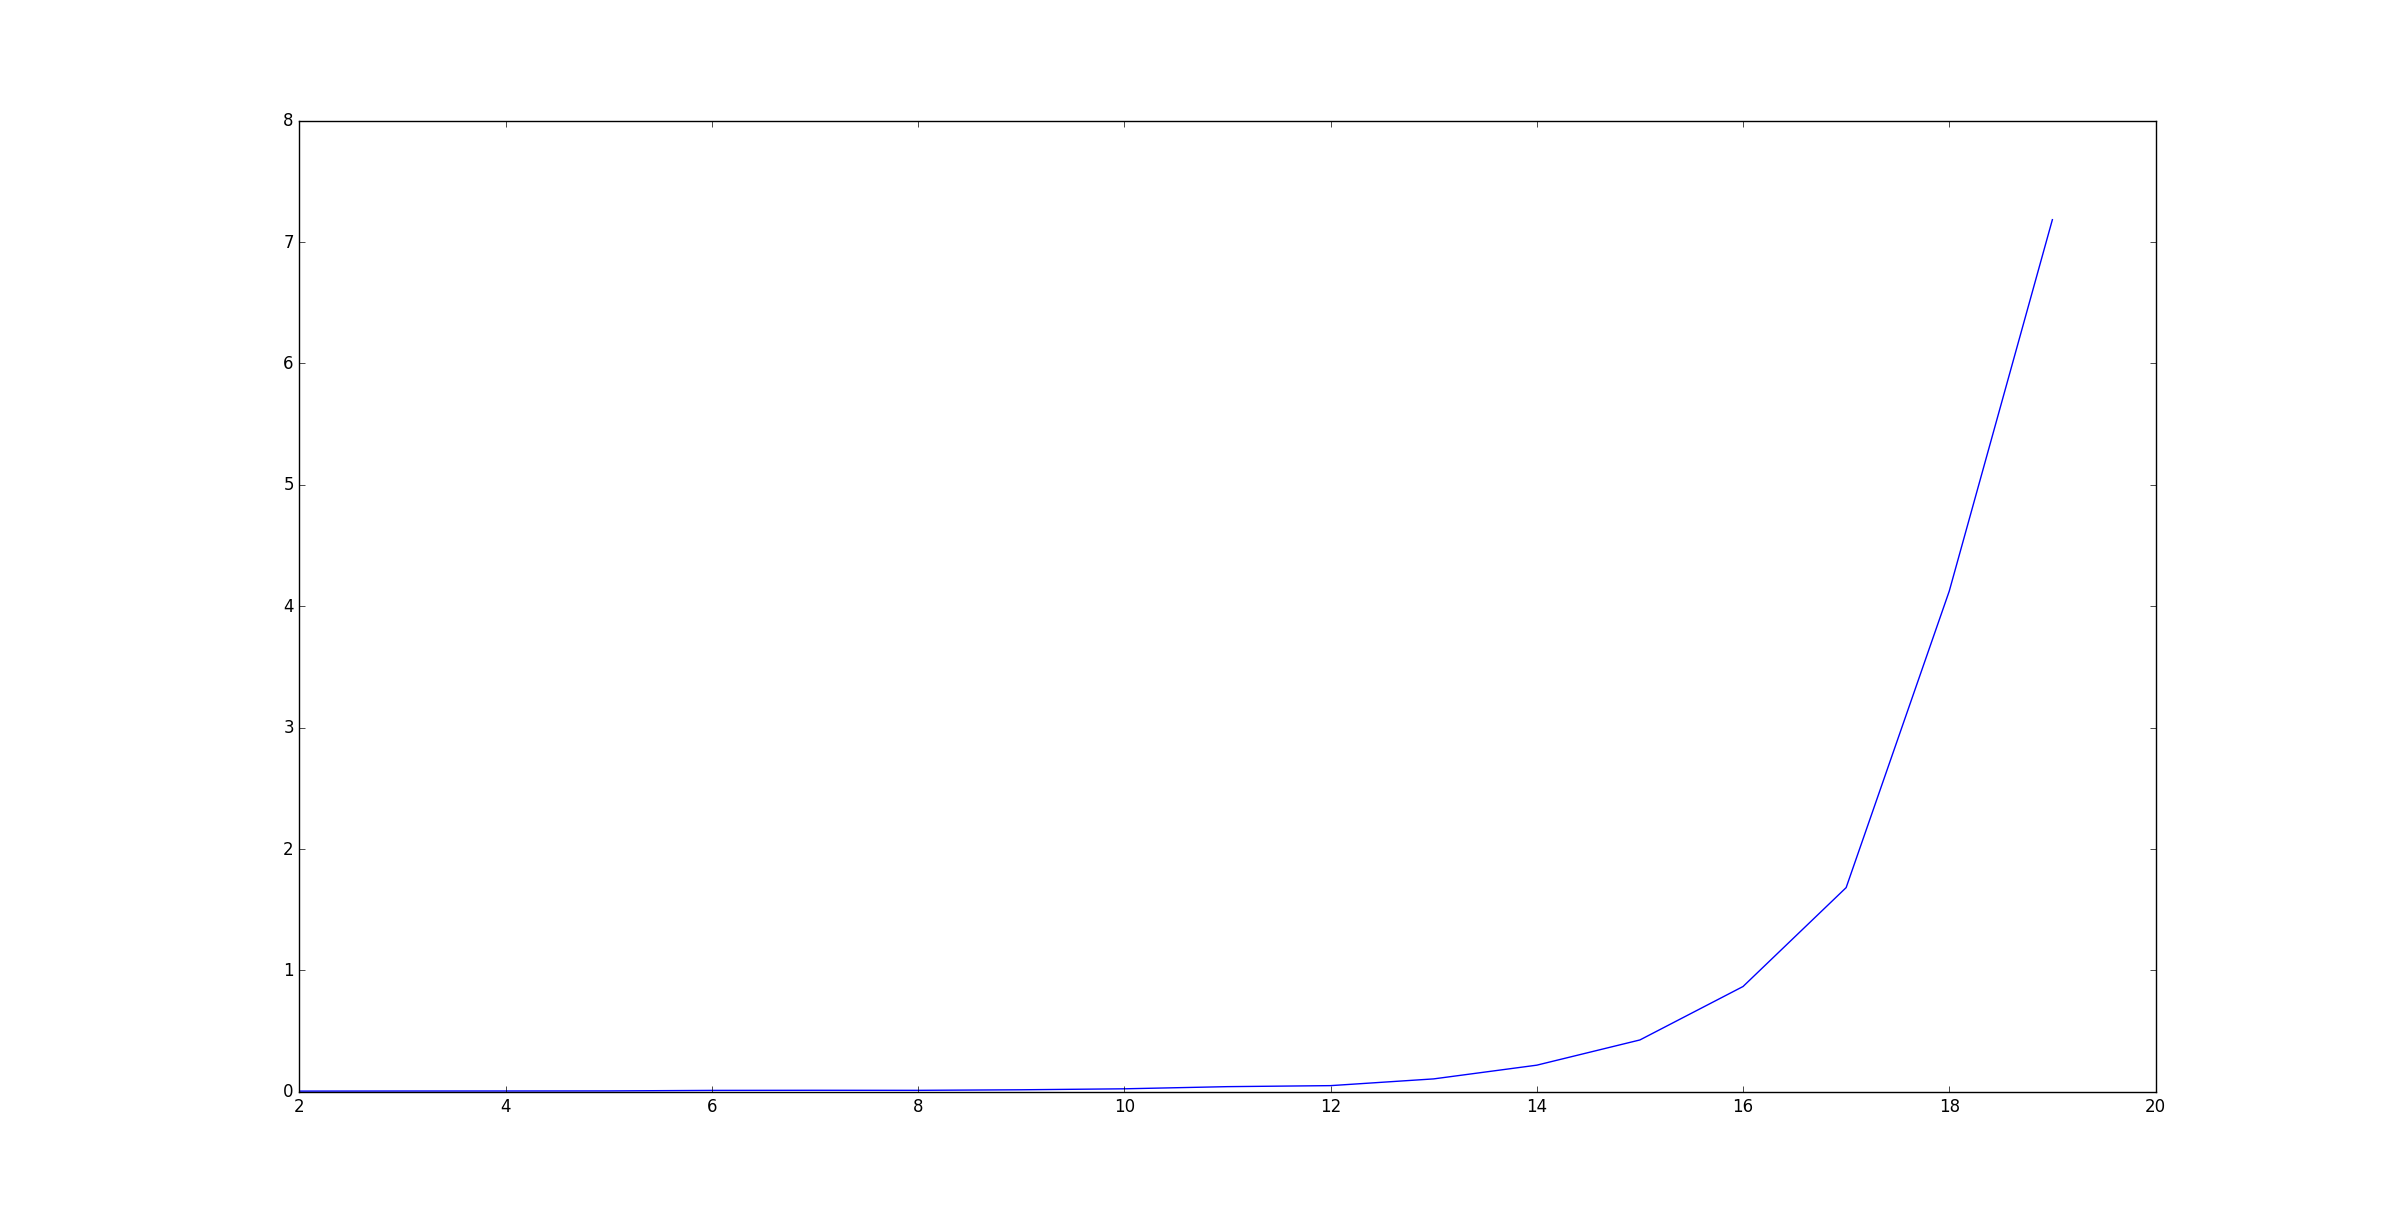
\includegraphics[width=450pt]{benchmark.png}
\end{center}

\section{Le sifting}
Cette partie a été réalisée par Joël Felderhoff.

Le plus gros problème que j'ai eu concernant le sifting a été de choisir la manière de le représenter en mémoire.
En effet, deux choix s'offraient à moi : soit utiliser des ``ref de ref'' ou émuler une mémoire directement dans OCaml. Après concertation avec Louis, j'ai choisi
cette deuxième option pour deux raisons. La première est que cela me posait problème d'utiliser des ref de ref (je trouvais cela assez sale dans l'idée). La deuxième était que cela me
paraissais un bon exercice et un bon défi de re-coder une gestion de la mémoire basique en OCaml (et ce fût en effet un bon défi).

\subsection{La structure robdd\_sifting}
J'ai choisi de créer un type d'enregistrement Caml pour gérer le sifting. L'idée est de faire les manipulations sur une structure personnelle, que je pourrais modifier tout au long de 
l'implémentation, pour ensuite générer l'objet de type ``robdd'' que mon collègue pourrait utiliser sans se poser de questions.

L'idée de mon type est de renommer dans un premier temps les variables pour ne travailler qu'avec des variables entre 1 et n.

Ensuite, on enregistre chaques noeud dans la mémoire, en lui associant bijectivement un entier : son index (comprendre ``adresse mémoire''). 

Puis, on garde en mémoire la taille de la robdd, qui sera modifiée par les ajouts et retraits de noeuds, et on crée une ``lvlTable'', qui stockera la liste de tous les noeuds correspondants à un 
littéral donné.

On garde également une table qui associe à chaque ``niveau'' du DAG un littéral (on commence avec le littéral i au niveau i)

Pour finir, l'index de la racine est conservé, pour la génération finale de l'arbre.

\subsection{Émulation de mémoire}
On garde toujours une bijection entre les noeuds et les entiers de case mémoire. L'idée est que lorsqu'on libère une case (avec la fonction ``free\_node'') on libère une case, qui est rajoutée à la liste des 
cases libres, prête à être utilisée quand on créera une nouvelle variable.

Je garde également dans ma structure le nombre de pointeur vers une certaine case mémoire : cela me permet de libérer un noeud du DAG uniquement lorsqu'il n'est plus pointé par aucun autre
noeud, comme recommandé dans l'article.

J'ai écrit différentes fonctions pour gérer la mémoire. Je ne vais pas toutes les lister car le code est commenté, mais les principales sont ``delete\_node'' qui supprime un noeud en mémoire, sans en libérer la
case et ``add\_node\_if\_not\_present'', dont le nom parle d'elle même.

\subsection{Le sifting en lui même}
Le plus gros travail a été sur l'émulation de mémoire en elle même. Le swapping m'a demandé principalement du travail de debug. L'article étudié ne précisais pas tous les cas possibles d'échanges, 
notamment lorsque les fils d'un noeud ne pointent pas vers le niveau suivant du DAG. Tous ces cas sont gérés, et on libére les noeuds qui ne sont plus utilisés, comme prévu dans l'article.

Une fois ce travail réalisé, le sifting n'est qu'une concaténation de 3 boucles dans 1 autre, cela ne m'a donc pas demandé beaucoup de travail.

\subsection{Résultats}
Quelques beaux résultats de réductions avec le sifting sont disponibles dans le fichier ``exemples\_sifting.txt''. On remarque une très bonne réduction pour gros exemples.

Je n'ai pas pus aller plus loin que 20 variables 150 clauses pour des raisons de temps.

\end{document}          
